\documentclass[a4paper, 12pt]{article}
\usepackage[top=1cm, bottom=2.1cm, left=2cm, right=2cm]{geometry}
\usepackage[utf8]{inputenc}
\usepackage{graphicx, caption}
\usepackage{float}
\usepackage{amsmath, amsfonts, amssymb, esint}
\usepackage{color}
\usepackage{hyperref}
\usepackage{multicol}
\usepackage{wallpaper}

\CenterWallPaper{1}{./img/background.png}

\definecolor{red}{rgb}{1,0,0}

\newcommand{\cabecalho}[4]
{
	\begin{figure}
		\centering
		\href{https://ligaolimpicadeastronomia.com.br/}{
\includegraphics[scale=0.6]{./img/logos.png}}
	\end{figure}
	
	\begin{center}
		\begin{large}
			\textbf{#1}	
		\end{large}
			\linebreak Listas OBA (Nível 4) -- #2ª Lista
			\linebreak #3
		\end{center}
	
	\begin{flushright}
		Material elaborado por \textbf{#4}
	\end{flushright}
}

\begin{document}
	\cabecalho{\textcolor{red}{Gabarito}}{1}{Terra, Lua e Sol}{Iago Braz Mendes}
	
	\begin{flushleft}
	\begin{itemize}
		\item \textbf{Questão 1) (1 ponto)} Os primeiros eclipses foram registados há cerca de 4 mil anos na Babilônia. Ao longo da história, eles provocaram medo e admiração. Ao observarem os eclipses, povos de diferentes épocas relacionaram esse fenômeno à intervenção de figuras mitológicas que tentariam devorar os astros e a sua luz.
			\begin{itemize}
				\item \textbf{Pergunta 1a) (0,5 ponto)} Analise as 2 astrofotos tiradas pelo autor desta lista :) e marque o item que mostra um eclipse.
					\begin{multicols}{2}
						\begin{figure}[H]
							\centering
							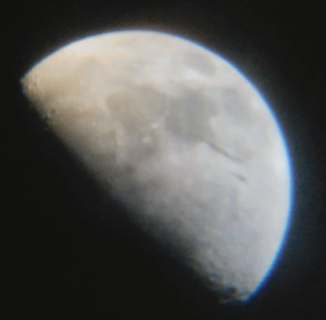
\includegraphics[width=.6\linewidth]{./img/1-cre.png}
							\captionsetup{labelformat=empty}
							\caption{(a)}
							\end{figure}
						\begin{figure}[H]
							\centering
							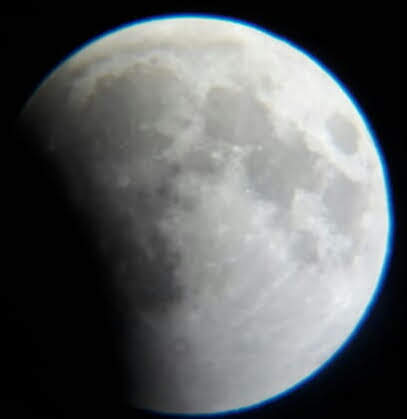
\includegraphics[width=.6\linewidth]{./img/1-ecl.jpg}
							\captionsetup{labelformat=empty}
							\caption{\textcolor{red}{(b)}}
						\end{figure}
					\end{multicols}
					\textcolor{red}{Perceba que, no item b, a parte escura está com um formato arredondado, o que só ocorre em eclipses. Inclusive, foi assim que, há muito tempo, Aristóteles sugeriu que a Terra devia ser redonda devido a sua sombra projetada na Lua.}
				\item \textbf{Pergunta 1b) (0.25 ponto)} Que tipo de eclipse é mostrado?
					\begin{itemize}
						\item[$(\textcolor{red}{X})$] Eclipse lunar
						\item[$(\quad)$] Eclipse solar
					\end{itemize}
					\textcolor{red}{A sombra da Terra está sendo projetada na Lua, então é um eclipse lunar. Só seria um eclipse solar caso a sombra do Sol estivesse sendo projetada na Terra.}
				\item \textbf{Pergunta 1c) (0.25 ponto)} Em qual fase lunar esse eclipse aconteceu?
					\begin{itemize}
						\item[$(\quad)$] Lua Nova
						\item[$(\quad)$] Lua Crescente
						\item[$(\textcolor{red}{X})$] Lua Cheia
						\item[$(\quad)$] Lua Minguante
					\end{itemize}
					\textcolor{red}{Eclipses lunares só podem ocorrer quando está Cheia, pois é preciso o alinhamento Sol-Terra-Lua. De modo análogo, eclipses solares só acontecem na Lua Nova, quando o alinhamento é Sol-Lua-Terra.}
			\end{itemize}
		\item \textbf{Questão 2) (1 ponto)} Analise, mais uma vez, a imagem do item que você \textbf{não} marcou como sendo um eclipse na questão anterior. Ela foi tirada no Hemisfério Sul por meio de um telescópio refletor. A imagem está exatamente como é observada na lente ocular, a qual produz uma imagem invertida.
			\begin{itemize}
				\item \textbf{Pergunta 2) (1 ponto)} Levando em consideração o que foi dito, em qual fase lunar essa foto foi tirada?
					\begin{itemize}
						\item[$(\quad)$] Lua Nova
						\item[$(\textcolor{red}{X})$] Lua Crescente
						\item[$(\quad)$] Lua Cheia
						\item[$(\quad)$] Lua Minguante
					\end{itemize}
					\textcolor{red}{Como a imagem está invertida, a face iluminada é a oeste (no hemisfério sul, o lado esquerdo). Dessa forma, podemos afirmar que a foto foi tirada na Lua Crescente. Se a face iluminada fosse a leste, a Lua seria Minguante.}
			\end{itemize}
		\item \textbf{Questão 3) (1 ponto)} 1 ano terrestre é comumente relacionado ao intervalo de tempo correspondente à translação completa da Terra em torno do Sol. Contudo, o valor exato de 1 ano varia de acordo com o método de análise. Nesse sentido, temos duas definições principais para essa medida de tempo: Ano Tropical e Ano Sideral.
			\begin{itemize}
				\item \textbf{Pergunta 3a) (0,25 ponto)} Qual o referencial na medida do Ano Tropical?
					\begin{itemize}
						\item[$(\quad)$] Movimento Retrógrado de Marte
						\item[$(\textcolor{red}{X})$] Equinócio Vernal (início das estações do ano)
						\item[$(\quad)$] Ápex (ponto para o qual o Sol se dirige)
						\item[$(\quad)$] Periélio ou Afélio
					\end{itemize}
					\textcolor{red}{O Ano Tropical é o intervalo de tempo entre duas passagens consecutivas do Sol pelo ponto Vernal -- ponto da Esfera Celeste onde se encontra o Sol no início das estações (equinócio de março).}
				\item \textbf{Pergunta 3b) (0,25 ponto)} Qual o referencial na medida do Ano Sideral?
					\begin{itemize}
						\item[$(\quad)$] Planetas do Sistema Solar
						\item[$(\quad)$] Galáxia de Andrômeda
						\item[$(\quad)$] Quasares
						\item[$(\textcolor{red}{X})$] Estrelas de Fundo
					\end{itemize}
					\textcolor{red}{O Ano Sideral é o intervalo de tempo entre duas passagens consecutivas do Sol pela mesma posição de acordo com as estrelas de fundo -- estrelas tão distantes que podem ser consideradas fixas na Esfera Celeste para distâncias pequenas como dentro do Sistema Solar.}
				\item \textbf{Pergunta 3c) (0,25 ponto)} O Ano Tropical tem duração de 365,2564 dias solares médios, enquanto o Ano Sideral possui 365,2422 dias solares médios. Qual é o \textbf{principal} movimento terrestre responsável por essa diferença?
					\begin{itemize}
						\item[$(\quad)$] Rotação da Terra
						\item[$(\quad)$] Translação da Terra
						\item[$(\textcolor{red}{X})$] Precessão dos Equinócios
						\item[$(\quad)$] Nutação
					\end{itemize}
					\textcolor{red}{A precessão dos equinócios é o movimento terrestre responsável por alterar a direção do eixo de rotação. Com isso, a relação entre as coordenadas celestes e eclípticas sofre pequenas alterações ao longo do seu período de 25.770 anos.}
				\item \textbf{Pergunta 3d) (0,25 ponto)} Geralmente, usamos 365,25 dias solares médios como uma aproximação para a duração do ano na Astronomia. Contudo, o nosso calendário possui 365 dias, o que deixa cerca de $\frac{1}{4}$ dia sobrando. Para consertar isso, temos o ano bissexto, o qual possui 366 dias solares médios e segue uma regra de 3 exigências. Pensando nisso, marque a seguir somente o(s) ano(s) que é(são) bissexto(s):
					\begin{itemize}
						\item[$(\textcolor{red}{X})$] 2400
						\item[$(\quad)$] 1846
						\item[$(\quad)$] 2100
						\item[$(\textcolor{red}{X})$] 1960
					\end{itemize}
					\textcolor{red}{Basta conferir as 3 exigências: 1) O ano deve ser múltiplo de 4; 2) O ano não pode ser múltiplo de 100; 3) A exigência 2 não vale, caso o ano seja múltiplo de 400.}
					\textcolor{red}
					{
						\begin{itemize}
							\item $2400$ é múltiplo de 4, de 100 e de 400. Portanto, é bissexto devido à exigência 3.
							\item $1846$ não é múltiplo de 4. Então, não é bissexto devido à exigência 1.
							\item $2100$ é múltiplo de 4 e de 100, e não é múltiplo de 400. Então, não é bissexto devido à exigência 2.
							\item $1960$ é múltiplo de 4. Então, é bissexto devido à exigência 1.
						\end{itemize}
					}
			\end{itemize}
		
		\item \textbf{Questão 4) (1 ponto)} Loinha -- uma estudante que usou muito o site da LOA -- foi medalhista de ouro na OBA e está atualmente estudando para as Seletivas. Em seus estudos, deparou-se com vários esquemas altazimutais e resolveu criar um com base no seu local de moradia. Assim, ela desenhou a seguinte representação:
			\begin{figure}[H]
				\centering
				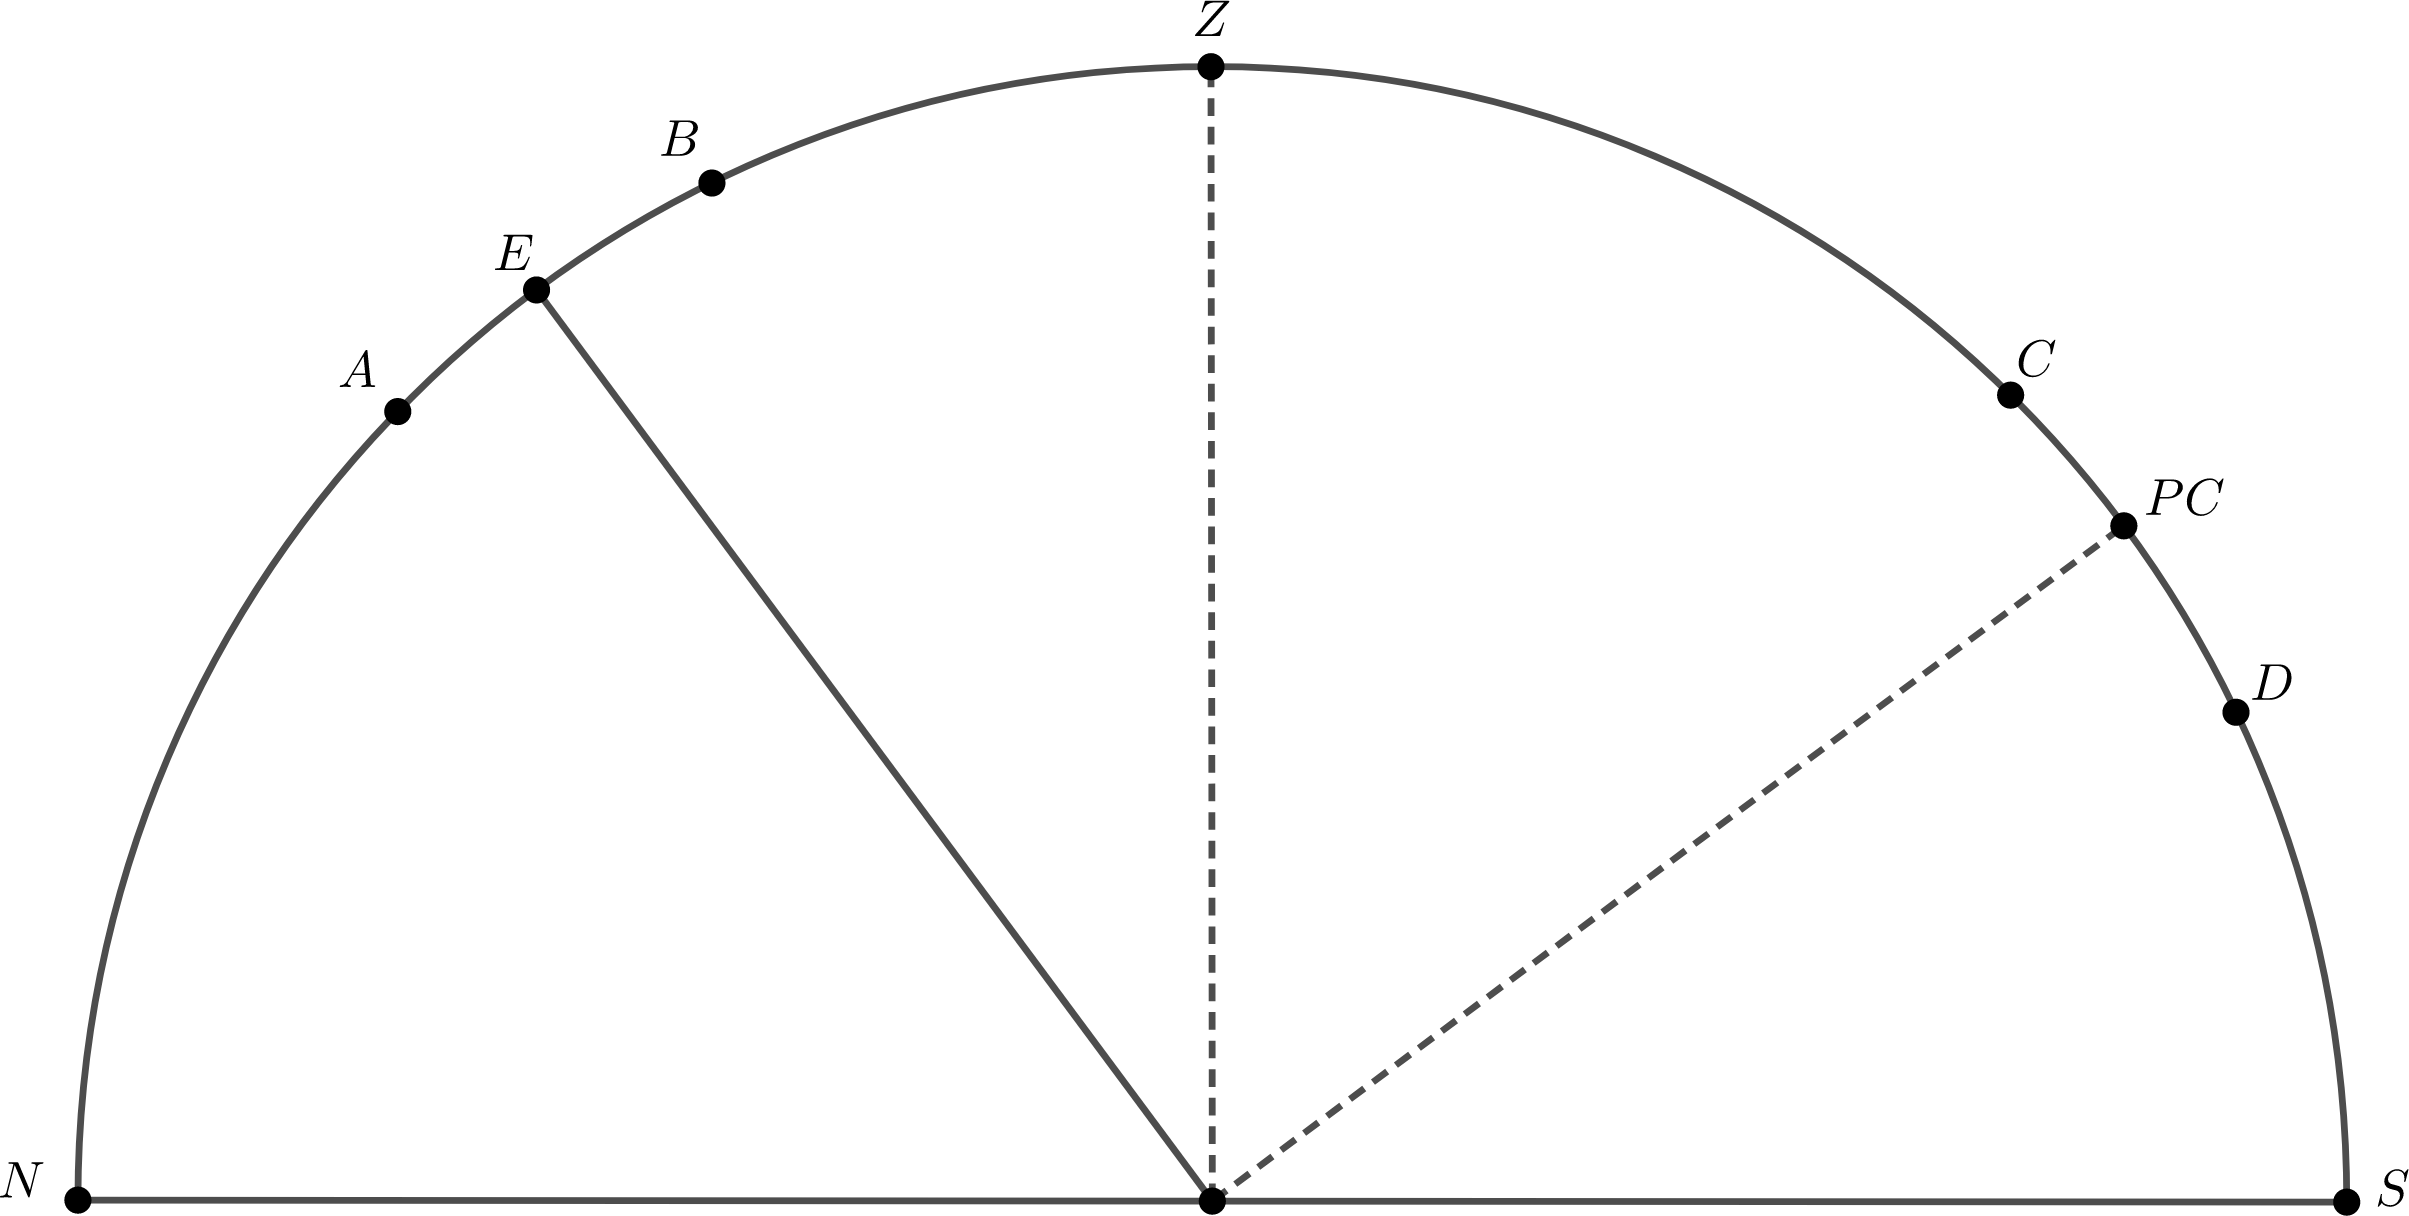
\includegraphics[scale=1.2]{./img/4.png}
			\end{figure}
			Nela, a linha horizontal representa o horizonte; o semiarco, a esfera celeste; $N$ e $S$, pontos cardeais norte e sul, respectivamente; $E$, o equador celeste (perceba que estamos olhando de lado, o que torna uma circunferência num segmento de reta); $PC$, o Polo Celeste elevado; $Z$, o zênite; e $A$, $B$, $C$ e $D$ pontos estratégicos na esfera celeste. \linebreak
			Como Loinha adora colocar em prática os conceitos aprendidos no site da LOA, fez alguns registros. Primeiramente, anotou a data e o horário: 22/06 (solstício de junho) ao meio-dia.\linebreak
			Observação: considere o mesmo horário para as perguntas.
			\begin{itemize}
				\item \textbf{Pergunta 4a) (0,5 ponto)} Depois, ele decidiu registrar em que posição o Sol se encontrava naquele momento. Qual a resposta correta?
					\begin{itemize}
						\item[$(\textcolor{red}{X})$] $A$
						\item[$(\quad)$] $B$
						\item[$(\quad)$] $C$
						\item[$(\quad)$] $D$
					\end{itemize}
					\textcolor{red}{No solstício de junho, o Sol está sobre o Trópico de Câncer, marcando o Verão no Hemisfério Norte e o Inverno no Hemisfério Sul. Portando, o Sol deve estar numa posição ao norte do Equador Celeste, o que só é verdade para $A$.}
					
				\item \textbf{Pergunta 4b) (0,5 ponto)} Animado para ver o comportamento das sombras, Loinha fincou uma haste na projeção do zênite no chão (centro da semicircunferência). Com a ajuda de uma bússola, anotou a direção cardeal para a qual a sombra apontava. Qual foi a anotação?
					\begin{itemize}
						\item[$(\quad)$] Norte
						\item[$(\quad)$] Leste
						\item[$(\textcolor{red}{X})$] Sul
						\item[$(\quad)$] Oeste
					\end{itemize}
					\textcolor{red}{Como o Sol está na direção Norte e no Meridiano Local (devido ao fato de ser meio-dia), a sombra deve apontar para a direção Sul.}
			\end{itemize}
		\item \textbf{Questão 5) (1 ponto)} Para as perguntas desta questão, considere o contexto da questão anterior.
			\begin{itemize}
				\item \textbf{Pergunta 5a) (0,5 ponto)} Em que lugar Loinha mora?
					\begin{itemize}
						\item[$(\quad)$] Hemisfério Norte
						\item[$(\quad)$] Equador
						\item[$(\textcolor{red}{X})$] Hemisfério Sul
					\end{itemize}
					\textcolor{red}{O polo elevado está apontando para a direção Sul, o que só ocorre no Hemisfério Sul. No Hemisfério Norte, o polo elevado aponta para a direção Norte e, no Equador, não há polo elevado.}
				\item \textbf{Pergunta 5b) (0,5 ponto)} No momento dos registros, que solstício estava ocorrendo no Hesisfério Norte e Sul, respectivamente?
					\begin{itemize}
						\item[$(\quad)$] Solstício de Verão e Solstício de Verão
						\item[$(\textcolor{red}{X})$] Solstício de Verão e Solstício de Inverno
						\item[$(\quad)$] Solstício de Inverno e Solstício de Inverno
						\item[$(\quad)$] Solstício de Inverno e Solstício de Verão
					\end{itemize}
					\textcolor{red}{Como o Sol está sobre o Trópico de Câncer, a insolação no Hemisfério Norte será maior do que no Hemisfério Sul. Portando, será Solstício de Verão naquele e de Inverno neste.}
			\end{itemize}
	\end{itemize}
	\end{flushleft}
\end{document}